\documentclass[a4paper,12pt]{article}
\usepackage{geometry}
\geometry{a4paper, margin=1in}

\usepackage{amsmath, amssymb}
\newcommand{\rvline}{\hspace*{-\arraycolsep}\vline\hspace*{-\arraycolsep}}
% See https://tex.stackexchange.com/questions/323297/typing-block-matrices-with-zero-blocks-and-separators
\usepackage{tikz}
\usetikzlibrary{quantikz2}

\usepackage{graphicx}
\usepackage{caption}

\usepackage{fancyhdr}
\usepackage{graphicx}
\usepackage{titlesec}
\usepackage{titling}
\usepackage{xcolor}
\usepackage{hyperref}
\hypersetup{
    colorlinks=true,
    linkcolor=blue,
    filecolor=magenta,      
    urlcolor=cyan,
}

% Header and Footer
\pagestyle{fancy}
\fancyhf{}
\fancyhead[L]{
\includegraphics[height=0.8cm]{logo.jpg}} % Include your institution logo
\fancyhead[C]{\footnotesize \textbf{\courseName}}
\fancyhead[R]{
\includegraphics[height=0.8cm]{ionq_logo_simple.png}}

\fancyfoot[L]{\projectName}
\fancyfoot[C]{Page \thepage}
\fancyfoot[R]{\today}

% Title formatting
\pretitle{\begin{center}\LARGE \bfseries}
\posttitle{\end{center}\vspace{0.5cm}}
\preauthor{\begin{center}\normalsize}
\postauthor{\end{center}}
\predate{\begin{center}\small}
\postdate{\end{center}\vspace{1cm}}

% Section formatting
\titleformat{\section}[block]{\Large\bfseries}{\thesection}{1em}{}
\titleformat{\subsection}[block]{\large\bfseries}{\thesubsection}{1em}{}
\titleformat{\subsubsection}[block]{\bfseries}{\thesubsubsection}{1em}{}

% Custom commands for student details
%\newcommand{\studentName}{Hyunseong Kim}
%\newcommand{\studentID}{20195048}
\newcommand{\courseName}{2024 IonQ summer Mentoring}
%\newcommand{\courseCode}{MM4020}
\newcommand{\assignmentTitle}{OptTrot}
%\newcommand{\dueDate}{June 30, 2024}

\newcommand{\projectName}{OptTrot}

\newtheorem{theorem}{Theorem}
\newtheorem{lemma}{Lemma}
\newtheorem{definition}{Definition}
\newtheorem{observation}{Observation}


\begin{document}

% Title Section
\begin{center}
%    %
\includegraphics[width=0.15\textwidth]{logo.png}\par\vspace{1cm} % Include your institution logo
%    {\scshape \courseName \par}
%    {Final Assignment \par}
%    \vspace{0.5cm}

    \vspace{0.5cm}
    {\Large\bfseries \assignmentTitle \par}
    {\large Optimized Trotter Circuit Library \par}
    \vspace{1cm}
    {
    \noindent
    \begin{minipage}{0.45\textwidth}
        \centering
        \textbf{Memebers}

        Hyunseong Kim

        Hanseo Kim
        
        Gaya Yun
    \end{minipage}
    \begin{minipage}{0.45\textwidth}
        \centering
        \textbf{Mentor}

        Sayomeo Ray
    \end{minipage}
    }
%    {\itshape \studentName \par}
%    {Student ID: \studentID \par}
%    \vspace{0.5cm}
%    {\large \today \par}
    \begin{abstract}
        OptTrot is a library of generating optimized Trotter circuit for a given hamiltonian.
        Trotterization is a standard way to accomplish time evolution circuit on gate model
        computer, however, their long depth circuit has significantly contributed to 
        the hurdle of practical application.
        In the library, we combined commuting partition method and Pauli Frame search method.
        If the given Pauli term mutually commuted with Pauli Frame axis, then the Clifford gate
        combination was reduced to combinations of CNOT gate. Moreoever their specific decomposition
        is easily derived from Gauss elimination of matrix over module 2 field.
    \end{abstract}
\end{center}


%\tableofcontents
%wpage

\section{Introduction}

OptTrot is a library for generating optimized Trotter circuits,
for practical use in various applications.

Trotterization is a standard method used to implement a time evolution operator 
by combining several local Hamiltonian evolution operators.
By using the method, we can expect the approximated operator closed to the original
operator, even the local terms did not commute with each other with quadratic, $O(t^2)$, error.

\begin{equation}
    \lim_{n \rightarrow \infty} (e^{A/2} e^{B/2})^n = e^{A+B}
\end{equation}

However, standard Trotterization method increases circuit depth with linear order 
by number of Pauli terms. That is, a hamiltonian whose number of local terms are $N$
has, at least, $N$ time deeper circuit than single Pauli term evolution circuit.
If the time evolution was an ultimate goal to achieve in quantum circuit, 
it could be meaningful, but in the most algorithms and applications, time evolution 
is just a part of the whole process. 
Thus, reducing techniques are significant to apply the quantum computer to general taskes.
In addition, increased circuit depth for reducing Trotter error yields 
inefficient costs in NISQ era, which makes the algorithm into less practical one.

By the limitation, there are many alternative methods to implement a time evolution operator 
with shorter depth circit than Trotterization, such as 
linear combination of unitary(LCU) method\cite{dewolf2023quantumcomputinglecturenotes}, Qubitization\cite{Low_2019}, 
Taylorization\cite{PhysRevLett.114.090502}, and Fractional query\cite{Berry_2014}.
Such methods make the evolution circuit more practical, however, they loose 
identity of the given system, especially the cases, when the given hamiltonian is nearly commute
or local observable was a dominant feature\cite{childs_theory_2021}. 
Only problem is a high cost of the Trotterization circuit. 
However, it is not a problem of Trotterization. 
It is a problem of circuit synthesis process of standard method\cite{nielsen2010quantum}.

\begin{figure}[!ht]
    \centering
    \begin{quantikz}
    & \gate{H} & \ctrl{1} & & \ctrl{1} & \gate{H} & \\
    &          & \targ{} & \gate{RZ}& \targ{} & & \\
    \end{quantikz}
    \label{fig:trotter_standard_circuit}
    \caption{Example of trotter evolution circuit. Where $H = X \otimes Z$}
\end{figure}

How can we optimize the circuit synthesis for trotter evolution circuit?
There have been various studies of circuit optimization, 
but for specificialy for trotter circuit. 
Schmitz et al would be a milestone paper\cite{schmitz_graph_2023}.
They analyzed what term would be rotated when we apply entanglement gates 
on quantum circuit and suggested a practical method to find a better depth
evolution circuit of given Hamiltonian.

Using Trotter error schema with commuting terms, 
we can analyze the overall error by applying order of local terms.

We will focus on attemption that author Kim's study, and 
combine them with Schmitz et al. 
The application of commuting partition to optimize 
the trotter circuit.

\subsection{Trotter Error by applying order}

It is well known that the exponential mapping error is represented with Baker Campbell Hausdorff formula.
Usually, the formula is not written with commutator form, Childs et al proved that the error term 
as a function of sequential commutator of local terms\cite{childs_theory_2021}.

\begin{equation}
    O(\alpha t^2)
\end{equation}

The results of Childs et al allow us to calculate 
the error boundary more precisely including a physical structure 
of the given Hamiltonian.

For example, let a given Hamiltonian was $H = c_i P_i + c_j P_j$.

\begin{equation}
    \exp(-it (c_i) P_i) \exp(-it (c_j) P_j) = \exp(- it (c_i P_i + c_j P_j)) + O (\alpha_{com}t^2)
\end{equation}

then the leading coefficient becomes $\alpha_{com} = \begin{cases}
    c_i + c_j & \mbox{ if } [P_i, P_j] = 0 \\
    c_i - c_j & \mbox{ if } [P_i, P_j] \neq 0 \\
\end{cases}$.

It is affected by coefficients, their size, and sign, and commutation property.
In the above example, we cannot observe the commutation and anti-commutation
effect, since, if they were commuting to each other, the $O(\alpha_{com} t^2) = 0$.
Let us expand the system to more general case.
Suppose that the given Hamiltonian has two representations,

\begin{align}
    H = H_1 + H_2 + H_3  \\
    H =  c_1 P_1 + c_2 P_2 + c_3 P_3 + c_4 P_4 + c_5 P_5\\
    H_1 = c_1 P_1 + c_3 P_3 \\
    H_2 = c_2 P_2\\
    H_3 = c_4 P_4 + c_5 P_5
\end{align}

where, $[H_i, H_j] \neq 0,$ and 
$[P_k, P_l] \neq 0$ if $P_k \in H_i, P_l \in H_j, i \neq j$.

\begin{align}
    \Pi_{l=1}^5 \exp(- i t (c_l P_l)) = \exp(-it H) + O(\alpha_{com 1} t^2)\label{eq:pauli_evolve}\\
    \Pi_{k=1}^3 \exp(- i t (H_k)) = \exp(-it H) + O(\alpha_{com 2} t^2) \label{eq:evolve_commute}
\end{align}


Following the $q=1$ order expansion, then in the first order, the bound error 
coefficients are reduced to 

\begin{align}
    \alpha_{com1} = 2(|| c_1 c_2 [P_1, P_2]|| + || c_1 c_4 [P_1, P_4]|| + || c_1 c_5 [P_1, P_5]||& \\
    + || c_2 c_3 [P_2, P_3]|| + || c_2 c_4 [P_2, P_4]|| + || c_2 c_5 [P_2, P_5]||& \\
    + || c_3 c_4 [P_3, P_4]|| + || c_3 c_5 [P_3, P_5]||)&\\
    \alpha_{com2} = 2(|| [H_1, H_2]|| + || [H_1, H_3]|| + || [H_2, H_3]||)& \\
\end{align}


\begin{align}
    0.5 \alpha_{com1} &= ||c_1 c_2|| + ||c_3 c_2|| + ||c_1 c_4|| + ||c_2 c_4|| + ||c_1 c_5|| + ||c_2 c_5||  + ||c_2 c_4|| + ||c_2 c_5||\\
    0.5 \alpha_{com2} &= ||c_1 c_2 + c_3 c_2|| + ||c_1 c_4 + c_2 c_4 + c_1 c_5 + c_2 c_5||  + ||c_2 c_4 + c_2 c_5||
\end{align}


Therefore, by the distribution of $\{c_i\}$ and commutation relationship of the local terms,
the constructed error rate vary.
However, Eq(\ref{eq:evolve_commute}) is just a re-ordering of Eq(\ref{eq:pauli_evolve}), since 

\begin{align}
    \exp(- i t (H_1)) &= \exp(- i t (c_1 P_1)) \exp(- i t (c_3 P_3)) \\ 
    \exp(- i t (H_2)) &= \exp(- i t (c_2 P_2))\\
    \exp(- i t (H_3)) &= \exp(- i t (c_4 P_4)) \exp(- i t (c_5 P_5)) \\ 
\end{align}

This is not et al, local Hamiltonian consist of mutually commuting Pauli terms provides us a lot of freedom
to optimize the circuit. 
Whatever we switch and reorder the Pauli terms in the applying trotter circuit,
if the larger structure, $\exp(-it H_j) = \Pi_k \exp(-it c_jk P_jk)$, was preserved then, 
the trotter error would be bounded while we reduce the number of gates in the implementation.
Thus, we don't have to choose one between trotter error and large gate error
to optimize the evolution circuit.

\textbf{Note}: The partitioning the hamiltonian into large local terms does not yields the optimized 
order in every situation. 
The term $\alpha$ only indicates upper bound of the error. So, the minimum trotter error could be 
worse than the arbitrary applying case. 
In here, the main focus is reducing errors associated with gate operations by using minimum
number of gates.



\section{Optimizing a circuit with commuting pairs}

Clique: optimal condition: sum $ \Sigma_{i} c_i \approx 0 $.

\subsection{Pauli Frame method}

One method to optimize the Trotter circuit is using \textit{Pauli Frame}\cite{schmitz_graph_2023}.
Pauli Frame is a collection of Pauli terms indicating axes on each quantum circuit wires
when we apply Rotation Z gate on the circuit.

\begin{figure}
    \centering
    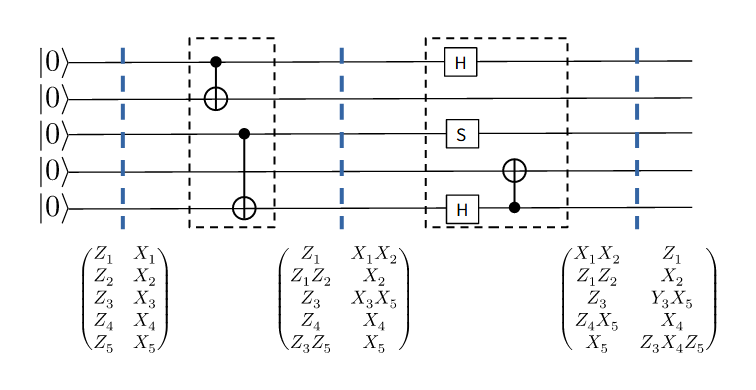
\includegraphics[width = 0.8\textwidth]{figures/Pauli Frame.png}
    \label{fig:Pauli Frame}
    \caption{
        Example of Pauli Frame analysis of a quantum circuit. 
        The dashed blue lines are corresponded to the below Pauli Frame.
        If we apply RZ gate on 5th qubit after we applied two CNOT gates,
        then the rotation gate is corresponding to $\exp(-i t Z_3Z_5)$.
    }
\end{figure}

Using the method, we can chase the what Pauli elements were applied, 
and what elements we can rotate on the circuit.




The current stage does not treat the routine finding 
optimal path search in Pauli Frame space.
It is because that we have not much tools to deal 
find the path and weight between the given frames,
excepting the dynamics programming approach.

The original paper formulated the problem as 
Traversal purchaser problem(TPP)\cite{schmitz_graph_2023}.
However, they did not solve the TPP problem and 
used a dynamic programming method to find a proper frame.
The reason is that, 
two calculate a distance between two frames, $B_i, B_j$, we have to know
all Frame information before we calculate.
However, what frame would be sufficient to represent a trotter path 
for the hamiltonian composites with entanglement gates?.
We cannot know the solution of such problem when arbitrary hamiltonian was given.
Moreover, when two frames were given, what Clifford gates would yields the 
transformation from $B_i$ to $B_j$?.
There is no solid frameworks to make the transformation.
The questions are remained from Schmitz et al paper.

\subsection{Path search over commuting cliques}

$I, Z$ family would be a good example to see the complxity
of the problem.
Consider that the local term of the Hamiltonian composite of $Z$ family.
Then, for a given frame $B$ and suppose that we have to make next frame to have $P = IIZZ$.
Since, we don't have to consider terms containing $X, Y$, we can simply write the term 
as single column, and the required entanglement gate is $CX$ gate only.

\begin{equation}
    B = \begin{bmatrix}
        ZZZI\\
        ZZIZ\\
        ZIZZ\\
        IZZZ
    \end{bmatrix}
    \rightarrow B' = \begin{bmatrix}
        IIZZ\\
        \dots\\
        \dots\\
        \dots
    \end{bmatrix}
\end{equation}


The answer is shotly applying a $CX$ gate on line 1 and 2.
The CNOT combination of $i, j$-th wires are identical to XOR of $w_i \oplus w_j$.

Now, let the representation as binary vector
\begin{equation}
B = \begin{bmatrix}
    ZZZI\\
    ZZIZ\\
    ZIZZ\\
    IZZZ
\end{bmatrix} = \begin{bmatrix}
    1110\\
    1101\\
    1011\\
    0111
\end{bmatrix} = 
\begin{bmatrix}
    \vec{w}_1\\
    \vec{w}_2\\
    \vec{w}_3\\
    \vec{w}_4
\end{bmatrix}
\end{equation}

Then the problem becomes the next statement.

\begin{quotation}
    \textit{Find the minimum size subgroup $\{w_k\} \subset B$ whose XOR products is $P$
    where, }

    \begin{equation}
        P = \wedge_{k} \vec{w}_k 
    \end{equation}

\end{quotation}

More simply, it is equivalent with finding a binary vector $\vec{x} \in \{0, 1\}^N$ of 

\begin{equation}
    P = \otimes_{i=1}^N x_i \& \vec{w}_i
\end{equation}

The solution could be derived with simple linear algebra on specific field, $\mathbb{Z}/2\mathbb{Z}$.
Logical \textit{XOR} and \textit{AND} operators form commuting field, $(\mathbb{Z}/2\mathbb{Z} ,\wedge , \&)$.
See the proof in Appendix \ref{appendix:modulo_field}. 
The Gauss elimination process yields an solution of the above problem.

Suppose that we have circuit of the state where the Pauli Frame representation was,

\begin{equation}
    B_i = \begin{pmatrix}
        w_1 &, \cdot \\
        w_2 &, \cdot \\
        w_3 &, \cdot \\
        w_4 &, \cdot \\
    \end{pmatrix},
    \,
    \begin{matrix}
        w_1 &= Z_2Z_3Z_4 &= ZZZI &= 1110_{sym}\\
        w_2 &= Z_1Z_3Z_4 &= ZZIZ &= 1101_{sym}\\
        w_3 &= Z_1Z_2Z_4 &= ZIZZ &= 1011_{sym}\\
        w_4 &= Z_1Z_2Z_3 &= IZZZ &= 0111_{sym}\\
    \end{matrix}
\end{equation}

and we want to apply $\exp(-i t Z1Z2)$ gate on circuit, what CNOT gate combination yieds
the quantum circuit state for the unitary operator, by simply applying RZ gate on a wire?
Luckily, XOR is commute aslike the CNOT gate becomes a conjugation of itself.
Let, $v =[1, 1, 0, 0]^T$, it is a symplectic representation of $Z_1Z_2$,
and $x = [x_1, x_2, x_3, x_4]^T, x_i \in \{0, 1\}$. 

\begin{equation}
    M x = v
\end{equation}

\begin{equation}
    M = \begin{bmatrix}
            & \rvline &     & \rvline &      & \rvline &  \\
        w_1 & \rvline &  w_2& \rvline &  w_3 & \rvline &  w_4\\
            & \rvline &     & \rvline &      & \rvline &  \\
    \end{bmatrix}
\end{equation}

\begin{equation} 
    \begin{bmatrix}
        0 & 1 & 1 & 1 \\
        1 & 0 & 1 & 1 \\
        1 & 1 & 0 & 1 \\
        1 & 1 & 1 & 0 \\
\end{bmatrix} \cdot \begin{bmatrix}
        x_1 \\
        x_2 \\
        x_3 \\
        x_4 \\
    \end{bmatrix} 
    = 
    \begin{bmatrix}
        1 \\
        1 \\
        0 \\
        0 \\
    \end{bmatrix}
\end{equation}

With Gauss elimination method, Reduced row echelon form would be obtained.

\begin{eqnarray}
    \begin{bmatrix}
        M &\rvline& v\\
    \end{bmatrix} \rightarrow 
    \begin{bmatrix}
        1 & 1 & 0 & 0 & \rvline & 0\\
        0 & 1 & 1 & 0 & \rvline & 1\\
        0 & 0 & 1 & 0 & \rvline & 0\\
        0 & 0 & 0 & 1 & \rvline & 0\\
    \end{bmatrix}
\end{eqnarray}


\begin{enumerate}
    \item $w_1 \oplus w_2 = 0$
    \item $w_2 \oplus w_3 = 1$
    \item $w_3 = 0$
    \item $w_4 = 0$
\end{enumerate}

Thus, we get $x = [1, 1, 0, 0]$, and


\begin{equation}
    [0, 1, 1, 1] \oplus [1, 0, 1, 1] = [1, 1, 0, 0]
\end{equation}

It means that CNOT over 1st and 2nd yeids $Z1Z2 = IIZZ$ Pauli element on the frame.

\begin{equation}
    B_i = \begin{pmatrix}
        ZZZI & \cdot \\
        ZZIZ & \cdot \\
        ZIZZ & \cdot \\
        IZZZ & \cdot \\
    \end{pmatrix}
    \rightarrow_{CNOT (1, 2)}
    B_{i+1} = \begin{pmatrix}
        ZZZI & \cdot \\
        \mathbf{IIZZ} & \cdot \\
        ZIZZ & \cdot \\
        IZZZ & \cdot \\
    \end{pmatrix}
\end{equation}

In general case, the local terms are not have the same properties 
of $IZ$ family terms, of course the same hold for $IX, IY$ families,
what about the rest of case?

\begin{observation}
For $N$ qubit system, the maximum size of mutually commuting Pauli subgroup, $P$, is $2^N$.
Let $G \subset P$ be a generator of $P$ where, $\forall p \in P, \exists \{g_i\} \subset G$
such that, $p = \wedge_i g_i$.
\end{observation}

\section{Mutually Commuting Paritition}

The remained question is how can we construct mutually commuting partition, 
from the given hamiltonian and its Pauli polynomial representation.
The answer is \textit{we cannot do that efficiently on classical computer}.
Suppose that we constructed a graph that indicates commuting relationship
of all Pauli terms in the hamiltonian. See Fig %\ref{}.

Partitioning the given Pauli elements is equivalent with \textit{Max-clique}
problem in computer science and it is a well-known NP-hard problem.

There are practical algorithms in many graph librarie%#\cite{} Networkx, Graph-tools, Rustworkx et cetra.
In addition, many quantum computer companies provide pratical solution for clique problems 
%D-Wave\cite{} 
%QuEra\cite{}

Which method is most practical method for the problem? 
Well, the answer is we don't know yet, sometimes quantum algorithm would show better result
with QAOA or anealing system,
but by the situation classic method would be better.
Choosing an algorithm is a job of researchers or users who want to generate optimized 
Trotter circuit. 
In here, providing a convenience interface would be enough.

\section{Conclusion}

In the report, we overlook the trotter error affected by order and hamiltonian structure 
in $n$-th order Suzukit-Trotter formula.

\appendix

\section{Proof of Modulo field}
\label{appendix:modulo_field}

$(\mathbb{Z}/2\mathbb{Z} ,\wedge , \&)$.

Denote, XOR($\wedge$) as $\oplus$ and, AND($\&$) as $\odot$,

\begin{equation}
    \begin{matrix}
        0 \oplus 0 & = &0\\
        0 \oplus 1 & = &1\\
        1 \oplus 0 & = &1\\
        1 \oplus 1 & = &0\\
    \end{matrix}
    \, 
    \begin{matrix}
        0 \odot 0 & = &0\\
        0 \odot 1 & = &0\\
        1 \odot 0 & = &0\\
        1 \odot 1 & = &1\\
    \end{matrix}
\end{equation}

Addition 

\begin{enumerate}
    \item a
\end{enumerate}

%Bibliography
\bibliographystyle{unsrt}  
\bibliography{references}  

\end{document}
